\newcommand\demodim{0.235\linewidth}

\begin{figure}\centering
	\caption{Example of \gridex{}'s hyper-cube partitioning (merging step not reported)}
	\subfloat[Surrounding\\cube]{
		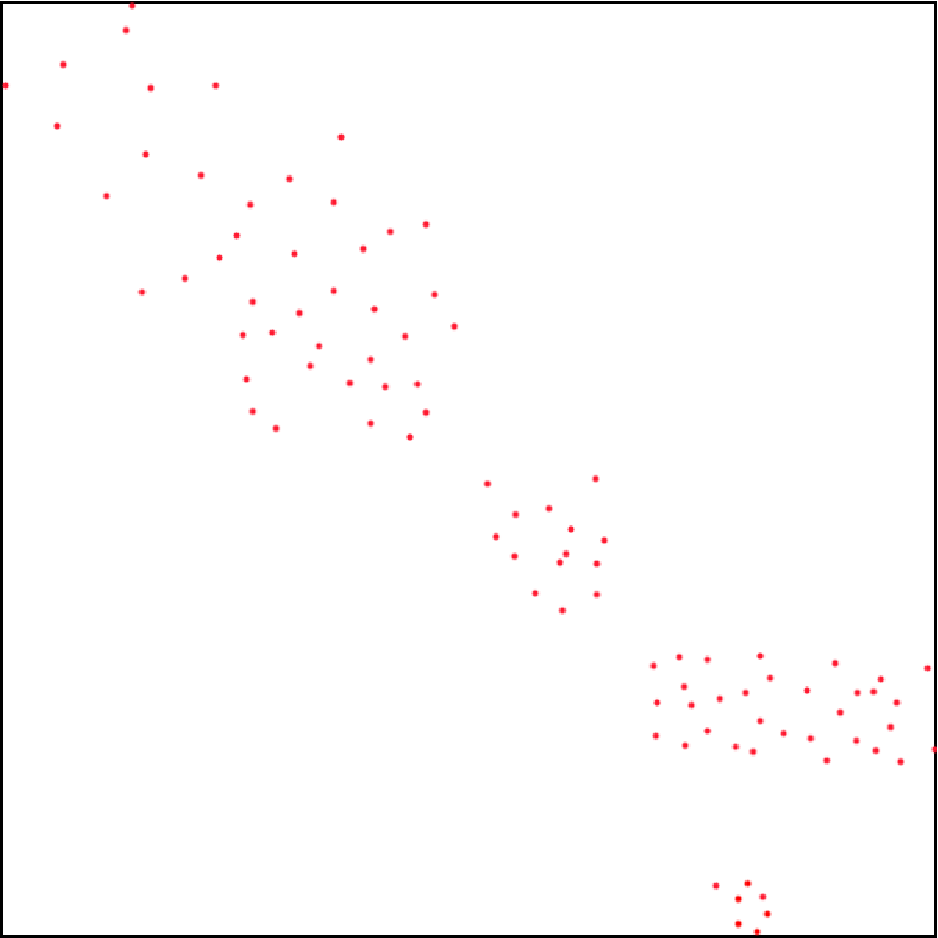
\includegraphics[width=\demodim]{figures/gridex/1.pdf}\label{fig:demo1}
	}
	\subfloat[Iteration 1 $(p_1=2)$]{
		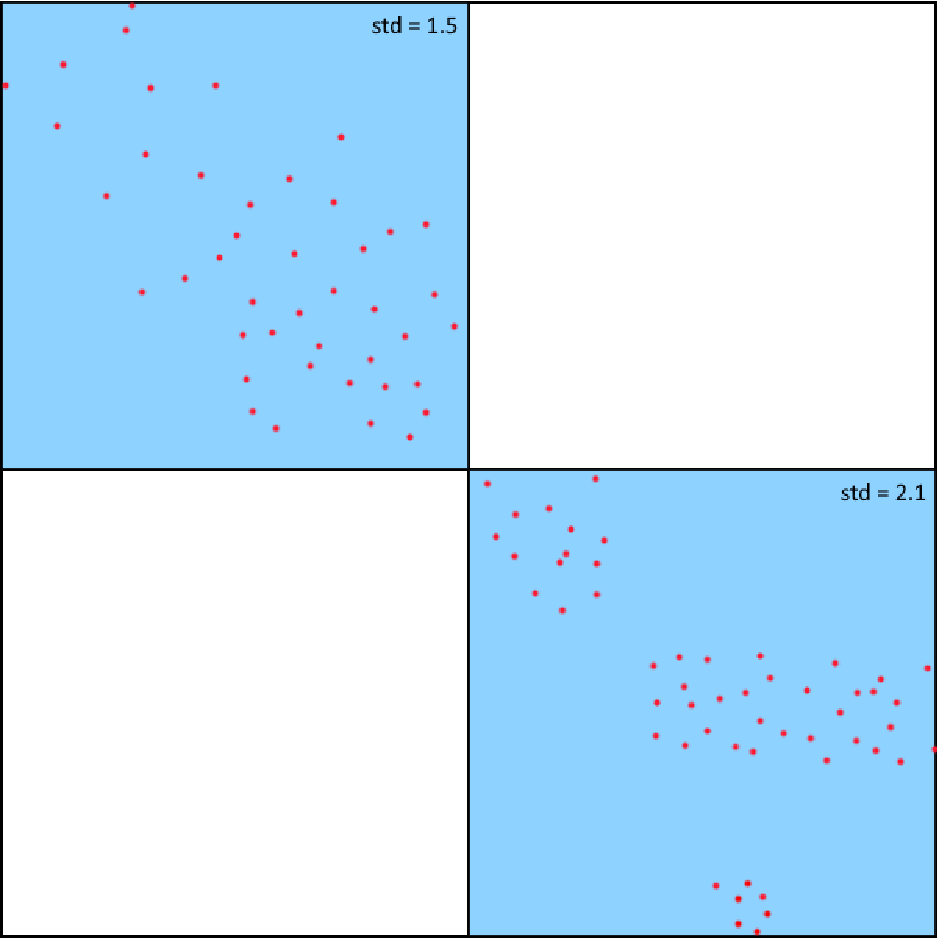
\includegraphics[width=\demodim]{figures/gridex/2.pdf}\label{fig:demo2}
	}
	\subfloat[Iteration 2 ($p_2 = 3$).]{
		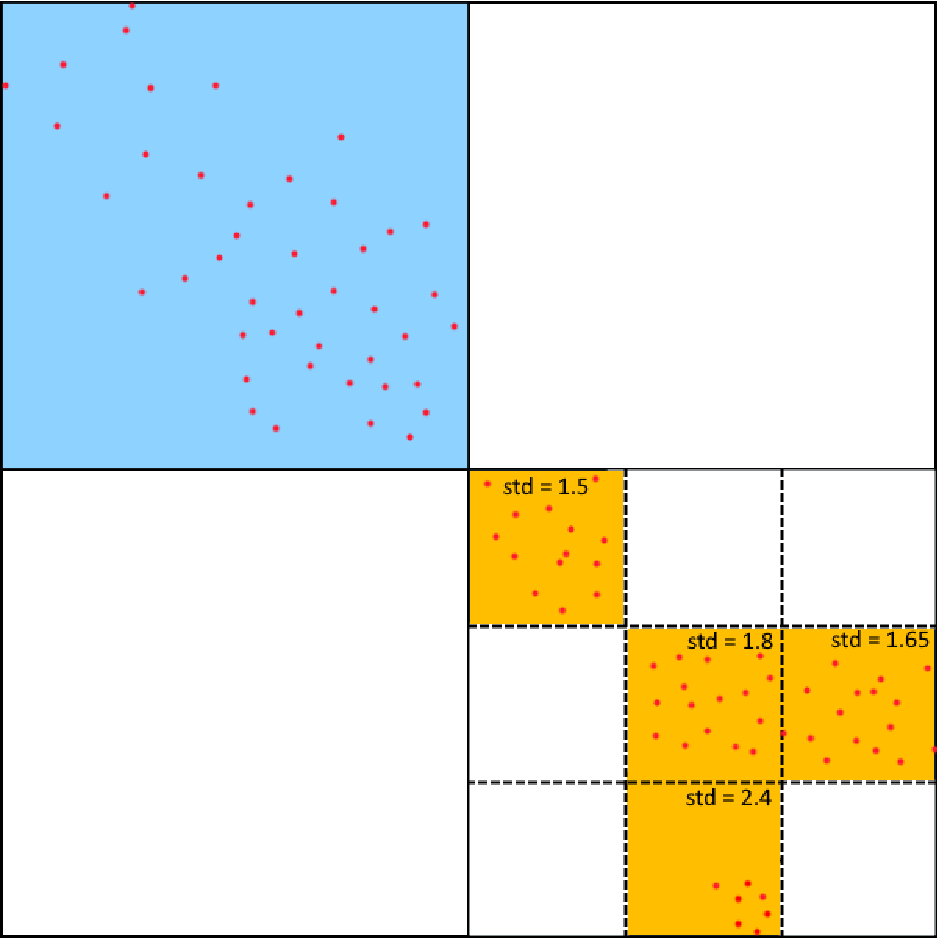
\includegraphics[width=\demodim]{figures/gridex/3.pdf}\label{fig:demo3}
	}
	\subfloat[Iteration 3 ($p_3 = 2$).]{
		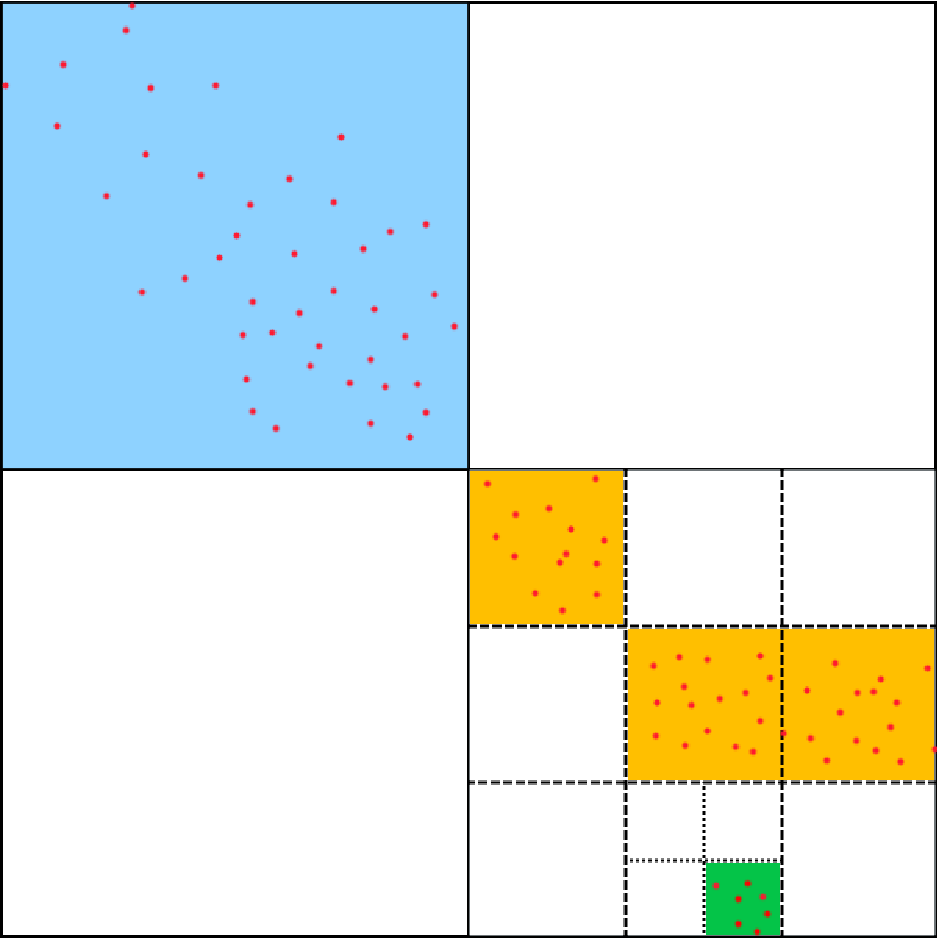
\includegraphics[width=\demodim]{figures/gridex/4.pdf}\label{fig:demo4}
	} 
\end{figure}
